% Build with XeLaTeX or LuaLaTeX for robust fonts and math
\documentclass{article}

% Layout and packages
\usepackage[a4paper,margin=2.5cm]{geometry}
\usepackage{amsmath, amssymb, amsthm}
\usepackage{bm}
\usepackage{hyperref}
\usepackage{graphicx}
\usepackage{caption}
\usepackage{listings}
\usepackage{xcolor}
\graphicspath{{figures/}}

% Code style
\lstdefinestyle{code}{
  basicstyle=\ttfamily\small,
  numbers=left,
  numberstyle=\tiny,
  numbersep=8pt,
  keywordstyle=\color{blue},
  commentstyle=\color{teal!70!black},
  stringstyle=\color{orange!70!black},
  showstringspaces=false,
  breaklines=true,
  frame=single,
  framerule=0.3pt,
  rulecolor=\color{black!15}
}
\lstset{style=code}

\title{Linear Regression: Theory, Formulas, Applications, and Practice}
\author{}
\date{\today}

\begin{document}
\maketitle
\tableofcontents

\section{Introduction}
Linear Regression is a fundamental supervised learning algorithm that models the linear relationship between input features and a continuous target. Thanks to its interpretability, efficiency, and closed-form solution, it is widely used as a baseline model and a quick validation tool in practice.

\section{Theory and Formulas}
\subsection{Model Assumption}
For a feature vector \(\mathbf{x} \in \mathbb{R}^d\), the model predicts
\begin{equation}
    \hat{y} = f(\mathbf{x}) = \mathbf{w}^\top \mathbf{x} + b,\quad \mathbf{w} \in \mathbb{R}^d,\; b \in \mathbb{R}.
\end{equation}
By augmenting features with a constant 1 and absorbing the bias into parameters, we write \(\hat{y} = \tilde{\mathbf{w}}^\top \tilde{\mathbf{x}}\).

\subsection{Matrix Form}
Given \(\mathbf{X}\in\mathbb{R}^{n\times d}\) and \(\mathbf{y}\in\mathbb{R}^{n}\), predictions are \(\hat{\mathbf{y}}=\mathbf{X}\mathbf{w}+b\mathbf{1}\). With augmented matrix \(\tilde{\mathbf{X}}=[\mathbf{X}\,\,\mathbf{1}]\) and \(\tilde{\mathbf{w}}=[\mathbf{w};b]\), we have \(\hat{\mathbf{y}}=\tilde{\mathbf{X}}\tilde{\mathbf{w}}\).

\subsection{Loss (Least Squares)}
We minimize the mean squared error (MSE):
\begin{equation}
    \mathcal{L}(\tilde{\mathbf{w}}) = \frac{1}{2n} \lVert \tilde{\mathbf{X}}\tilde{\mathbf{w}} - \mathbf{y} \rVert_2^2.
\end{equation}

\subsection{Closed-form (Ordinary Least Squares)}
If \(\tilde{\mathbf{X}}^\top\tilde{\mathbf{X}}\) is invertible, the optimum is
\begin{equation}
    \tilde{\mathbf{w}}^* = \big(\tilde{\mathbf{X}}^\top\tilde{\mathbf{X}}\big)^{-1}\tilde{\mathbf{X}}^\top\mathbf{y}.
\end{equation}
Numerically, QR or SVD is often preferred for stability.

\subsection{Gradient Descent (Optional)}
One can also use first-order optimization:
\begin{align}
    \nabla_{\tilde{\mathbf{w}}} \mathcal{L} &= \frac{1}{n} \tilde{\mathbf{X}}^\top\big(\tilde{\mathbf{X}}\tilde{\mathbf{w}} - \mathbf{y}\big),\\
    \tilde{\mathbf{w}} &\leftarrow \tilde{\mathbf{w}} - \eta\, \nabla_{\tilde{\mathbf{w}}} \mathcal{L},
\end{align}
with learning rate \(\eta\).

\subsection{Regularization (Optional)}
Ridge (L2) regression adds
\begin{equation}
    \min_{\tilde{\mathbf{w}}}\; \frac{1}{2n}\lVert \tilde{\mathbf{X}}\tilde{\mathbf{w}}-\mathbf{y}\rVert_2^2 + \frac{\lambda}{2}\lVert \mathbf{w}\rVert_2^2,
\end{equation}
with closed form \(\tilde{\mathbf{w}}^* = (\tilde{\mathbf{X}}^\top\tilde{\mathbf{X}} + \lambda\mathbf{I})^{-1}\tilde{\mathbf{X}}^\top\mathbf{y}\).

\section{Applications and Tips}
\begin{itemize}
  \item \textbf{Numerical forecasting}: Prices, sales, temperature and other continuous targets.
  \item \textbf{Interpretable baseline}: Coefficient magnitude/sign hints at feature impact.
  \item \textbf{Practical tips}: Feature scaling, outlier handling, multicollinearity diagnostics, CV for regularization.
\end{itemize}

\section{Python Practice: Closed-form Fit and Visualization}
This example will:
\begin{enumerate}
  \item Generate 1D linear data with noise;
  \item Fit via the augmented-matrix OLS closed form;
  \item Plot scatter and fitted line, saved to \texttt{figures/linear\_regression\_fit.png}.
\end{enumerate}

\begin{lstlisting}[language=Python,caption={linear_regression_closed_form.py}]
import os
import numpy as np
import matplotlib.pyplot as plt

np.random.seed(42)

# 1) Generate data: y = 3x + 2 + noise
n = 80
X = np.linspace(-3, 3, n).reshape(-1, 1)
true_w, true_b = 3.0, 2.0
y = true_w * X[:, 0] + true_b + np.random.normal(0, 1.0, size=n)

# 2) Augmented matrix and closed form
X_aug = np.hstack([X, np.ones((n, 1))])  # [x, 1]
theta = np.linalg.pinv(X_aug.T @ X_aug) @ X_aug.T @ y
w_hat, b_hat = theta[0], theta[1]

# 3) Visualization and save
fig, ax = plt.subplots(figsize=(6, 4))
ax.scatter(X[:, 0], y, s=18, alpha=0.7, label='data')
xx = np.linspace(X.min(), X.max(), 200)
yy = w_hat * xx + b_hat
ax.plot(xx, yy, color='crimson', lw=2.0, label=f'fit: y={w_hat:.2f}x+{b_hat:.2f}')
ax.set_xlabel('x')
ax.set_ylabel('y')
ax.legend()
ax.set_title('Linear Regression (Closed-form OLS)')

os.makedirs('figures', exist_ok=True)
out_path = os.path.join('figures', 'linear_regression_fit.png')
plt.tight_layout()
plt.savefig(out_path, dpi=160)
print('saved to', out_path)
\end{lstlisting}

\section{Result}
Figure~\ref{fig:fit} shows the fitted line against noisy samples.

\begin{figure}[h]
  \centering
  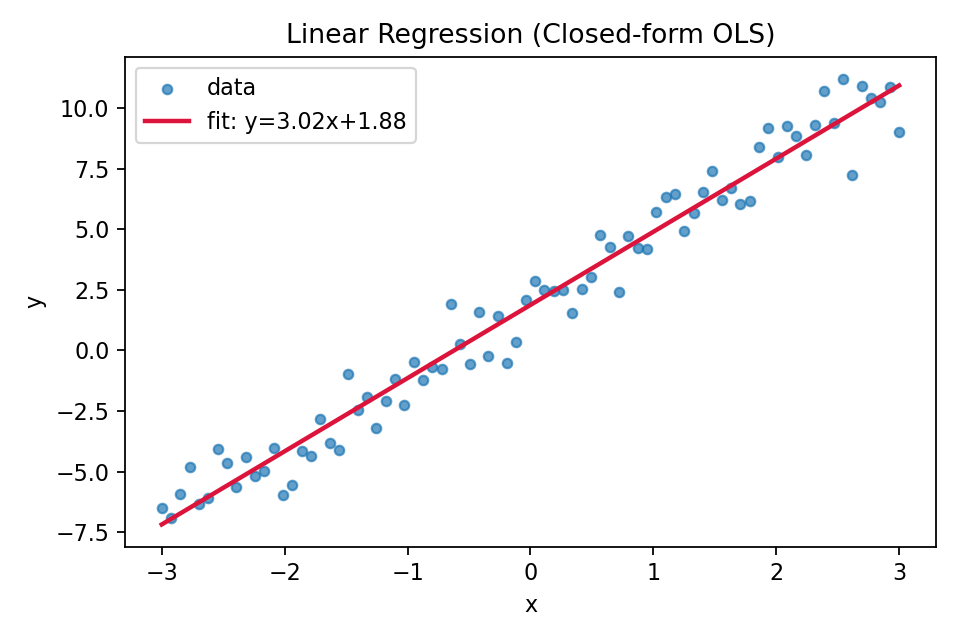
\includegraphics[width=0.75\linewidth]{linear_regression_fit.png}
  \caption{Linear regression fit on synthetic data}
  \label{fig:fit}
\end{figure}

\section{Summary}
Linear Regression is a simple yet powerful baseline. In practice, pay attention to scaling, outliers, and multicollinearity, and select regularization via cross-validation for robust generalization.

\end{document}

